\documentclass[11pt]{article}
\usepackage[margin=12mm,landscape]{geometry}
\usepackage[T1]{fontenc}
\usepackage{lmodern}
\usepackage{xcolor}
\usepackage{tikz}
\usetikzlibrary{arrows.meta,backgrounds,calc,fit,positioning,shapes.geometric}
\pagestyle{empty}

\definecolor{ink}{HTML}{1B2A2F}
\definecolor{teal}{HTML}{0F4C5C}
\definecolor{sage}{HTML}{DCE8E2}
\definecolor{amber}{HTML}{E8A33D}
\definecolor{coral}{HTML}{D9544D}
\definecolor{paper}{HTML}{FAF7F2}
\definecolor{line}{HTML}{D8D2C6}

\tikzset{
  font=\sffamily,
  flow/.style={-{Latex[length=2.2mm]},line width=1.1pt,draw=teal},
  data/.style={-{Latex[length=2mm]},line width=.8pt,draw=ink!55},
  box/.style={rounded corners=3mm,draw=line,line width=.8pt,fill=white,minimum height=15mm,align=center,inner sep=4mm},
  module/.style={box,draw=teal,line width=1.2pt,minimum width=45mm},
  proof/.style={box,draw=amber,fill=amber!10,minimum width=39mm},
  stop/.style={box,draw=coral,fill=coral!9,line width=1.2pt},
  badge/.style={rounded corners=2mm,fill=sage,draw=teal!35,inner xsep=2.5mm,inner ysep=1.2mm,font=\sffamily\scriptsize},
  title/.style={font=\sffamily\bfseries\Large,text=ink},
  subtitle/.style={font=\sffamily\small,text=ink!70,align=center}
}

\begin{document}
\begin{center}\tikz\node[title]{From visible work to transferable judgment};\quad
\tikz\node[badge]{Challenge walkthrough: Capture $\rightarrow$ Map $\rightarrow$ Teach};\end{center}

\begin{center}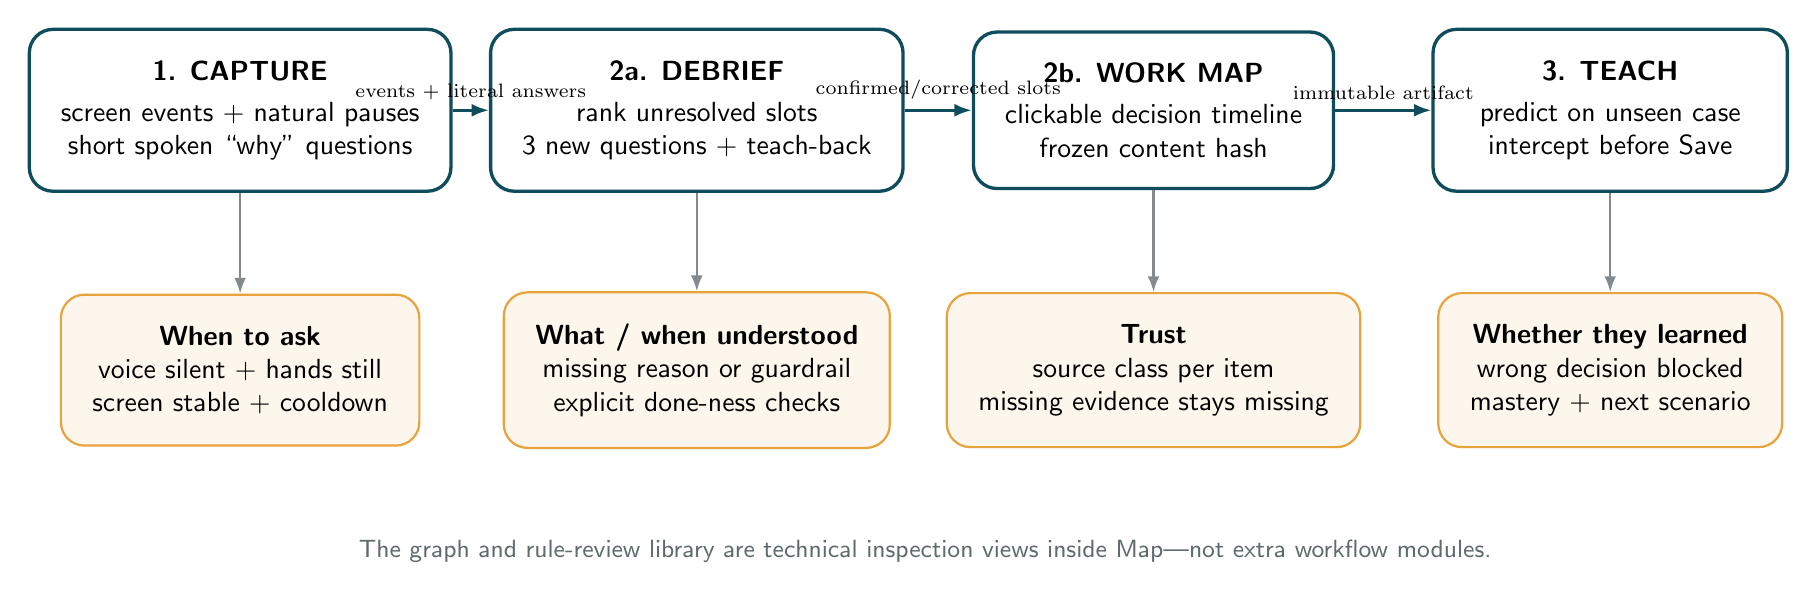
\begin{tikzpicture}
\node[module] (capture) at (-8.7,0) {\textbf{1. CAPTURE}\\[1mm]screen events + natural pauses\\short spoken ``why'' questions};
\node[module] (debrief) at (-2.9,0) {\textbf{2a. DEBRIEF}\\[1mm]rank unresolved slots\\3 new questions + teach-back};
\node[module] (map) at (2.9,0) {\textbf{2b. WORK MAP}\\[1mm]clickable decision timeline\\frozen content hash};
\node[module] (teach) at (8.7,0) {\textbf{3. TEACH}\\[1mm]predict on unseen case\\intercept before Save};
\draw[flow] (capture) -- node[above,font=\scriptsize]{events + literal answers} (debrief);
\draw[flow] (debrief) -- node[above,font=\scriptsize]{confirmed/corrected slots} (map);
\draw[flow] (map) -- node[above,font=\scriptsize]{immutable artifact} (teach);

\node[proof] (when) at (-8.7,-3.3) {\textbf{When to ask}\\voice silent + hands still\\screen stable + cooldown};
\node[proof] (what) at (-2.9,-3.3) {\textbf{What / when understood}\\missing reason or guardrail\\explicit done-ness checks};
\node[proof] (transfer) at (2.9,-3.3) {\textbf{Trust}\\source class per item\\missing evidence stays missing};
\node[proof] (learned) at (8.7,-3.3) {\textbf{Whether they learned}\\wrong decision blocked\\mastery + next scenario};
\draw[data] (capture) -- (when); \draw[data] (debrief) -- (what);
\draw[data] (map) -- (transfer); \draw[data] (teach) -- (learned);

\node[subtitle] at (0,-5.6) {The graph and rule-review library are technical inspection views inside Map---not extra workflow modules.};
\end{tikzpicture}\end{center}
\clearpage

\begin{center}\tikz\node[title]{Provenance: preserve differences, never flatten them};\end{center}
\begin{center}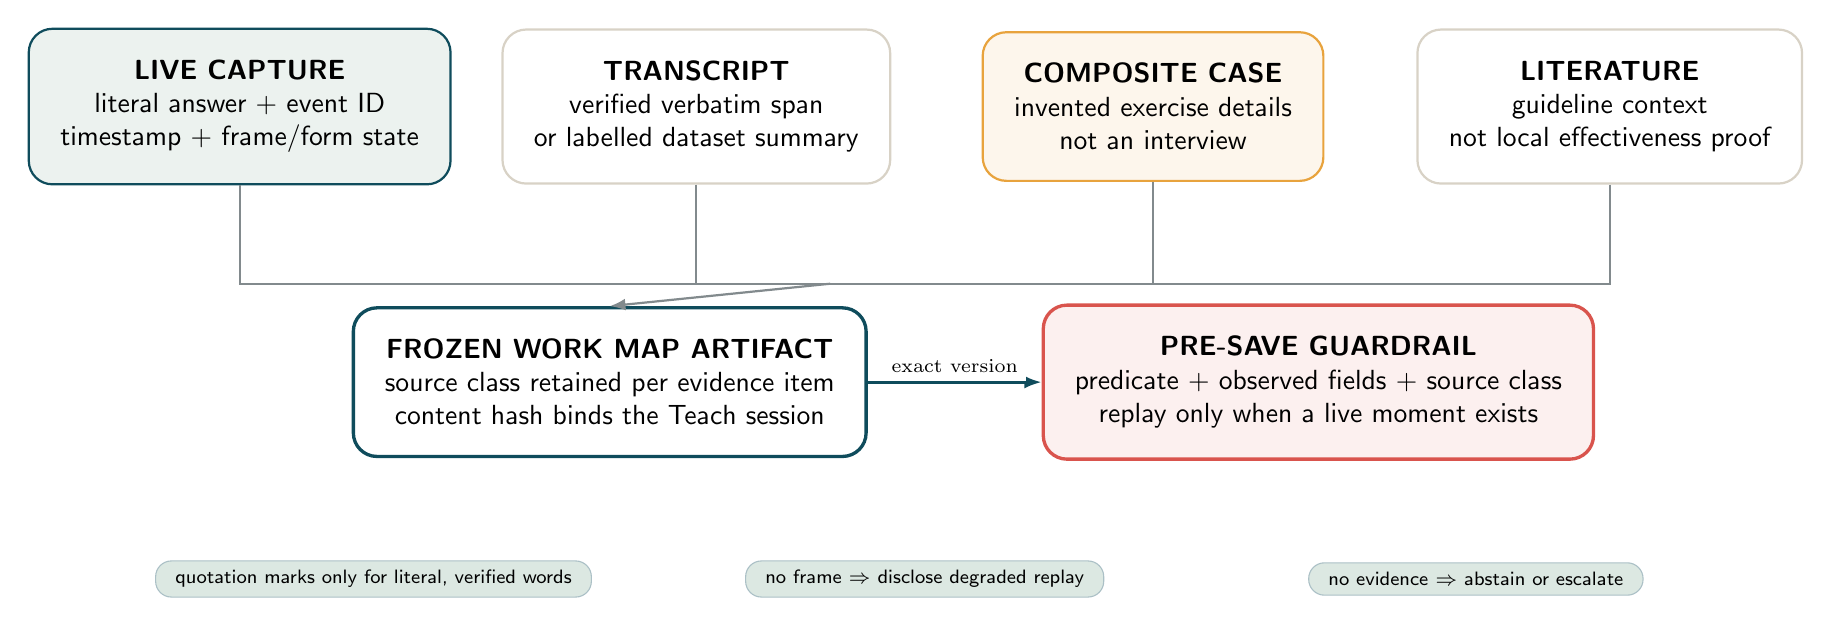
\begin{tikzpicture}
\node[box,draw=teal,fill=sage!55] (live) at (-8.7,0) {\textbf{LIVE CAPTURE}\\literal answer + event ID\\timestamp + frame/form state};
\node[box] (transcript) at (-2.9,0) {\textbf{TRANSCRIPT}\\verified verbatim span\\or labelled dataset summary};
\node[box,draw=amber,fill=amber!10] (composite) at (2.9,0) {\textbf{COMPOSITE CASE}\\invented exercise details\\not an interview};
\node[box] (literature) at (8.7,0) {\textbf{LITERATURE}\\guideline context\\not local effectiveness proof};

\node[module,minimum width=65mm] (artifact) at (-4,-3.5) {\textbf{FROZEN WORK MAP ARTIFACT}\\source class retained per evidence item\\content hash binds the Teach session};
\node[stop,minimum width=62mm] (guard) at (5,-3.5) {\textbf{PRE-SAVE GUARDRAIL}\\predicate + observed fields + source class\\replay only when a live moment exists};

\coordinate (merge) at (-1.2,-2.25);
\draw[data,-] (live.south) |- (merge); \draw[data,-] (transcript.south) |- (merge);
\draw[data,-] (composite.south) |- (merge); \draw[data,-] (literature.south) |- (merge);
\draw[data] (merge) -- (artifact.north);
\draw[flow] (artifact) -- node[above,font=\scriptsize,fill=white,inner sep=1mm]{exact version} (guard);

\node[badge] (rule1) at (-7,-6) {quotation marks only for literal, verified words};
\node[badge] (rule2) at (0,-6) {no frame $\Rightarrow$ disclose degraded replay};
\node[badge] (rule3) at (7,-6) {no evidence $\Rightarrow$ abstain or escalate};
\end{tikzpicture}\end{center}
\clearpage

\begin{center}\tikz\node[title]{Wandering demo: teach the method, then test transfer};\end{center}
\begin{center}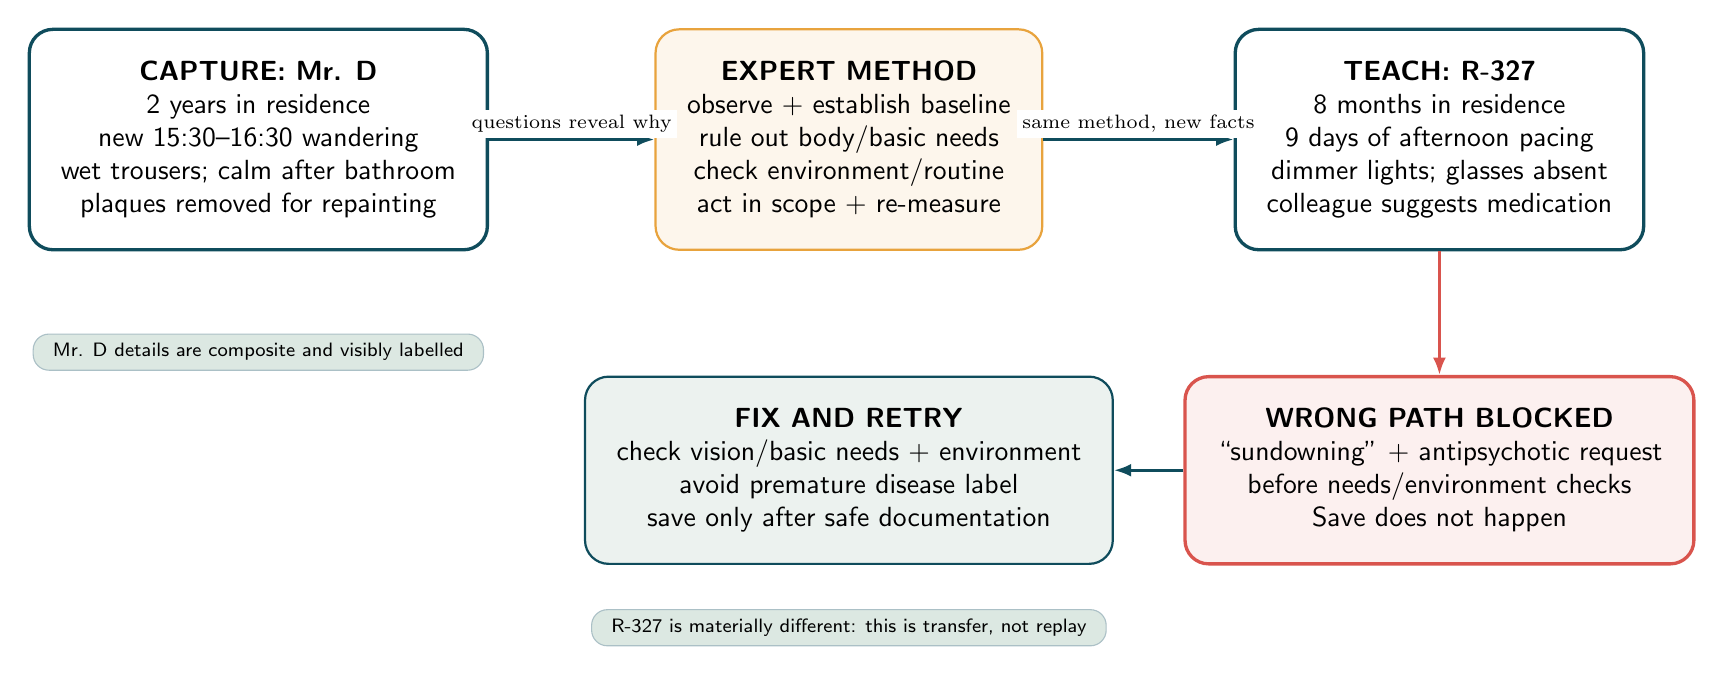
\begin{tikzpicture}
\node[module,minimum width=50mm] (mrD) at (-7.5,0) {\textbf{CAPTURE: Mr. D}\\2 years in residence\\new 15:30--16:30 wandering\\wet trousers; calm after bathroom\\plaques removed for repainting};
\node[proof,minimum width=47mm] (reason) at (0,0) {\textbf{EXPERT METHOD}\\observe + establish baseline\\rule out body/basic needs\\check environment/routine\\act in scope + re-measure};
\node[module,minimum width=50mm] (r327) at (7.5,0) {\textbf{TEACH: R-327}\\8 months in residence\\9 days of afternoon pacing\\dimmer lights; glasses absent\\colleague suggests medication};
\draw[flow] (mrD) -- node[above,font=\scriptsize,fill=white,inner sep=.7mm]{questions reveal why} (reason);
\draw[flow] (reason) -- node[above,font=\scriptsize,fill=white,inner sep=.7mm]{same method, new facts} (r327);

\node[stop,minimum width=58mm] (blocked) at (7.5,-4.2) {\textbf{WRONG PATH BLOCKED}\\``sundowning'' + antipsychotic request\\before needs/environment checks\\Save does not happen};
\node[box,draw=teal,fill=sage!55,minimum width=58mm] (fix) at (0,-4.2) {\textbf{FIX AND RETRY}\\check vision/basic needs + environment\\avoid premature disease label\\save only after safe documentation};
\draw[flow,draw=coral] (r327) -- (blocked);
\draw[flow] (blocked) -- (fix);

\node[badge] at (-7.5,-2.7) {Mr. D details are composite and visibly labelled};
\node[badge] at (0,-6.2) {R-327 is materially different: this is transfer, not replay};
\end{tikzpicture}\end{center}
\end{document}
